\chapter{Score Component Distributions}
\label{app:score_distributions}

This appendix contains the empirical distributions of the score components---volume term $\ln A_c$, shape term $d_{\mathrm{mah}}$, and final log-likelihood---for all three benchmarks (CIFAR-100, Caltech-256, ImageNet-R) and both covariance estimators (Diag-Cov and Full-Cov), computed separately on the training and validation splits. The two CIFAR-100 validation figures are shown in the main text (Figures~\ref{fig:hist_cifar_val} and~\ref{fig:hist_cifar_val_full}); the remaining figures are collected here for completeness.

% =============================================
% Diag-Cov: Training splits
% =============================================

\section*{Diagonal Covariance --- Training Splits}

\begin{figure}[htbp]
	\centering
	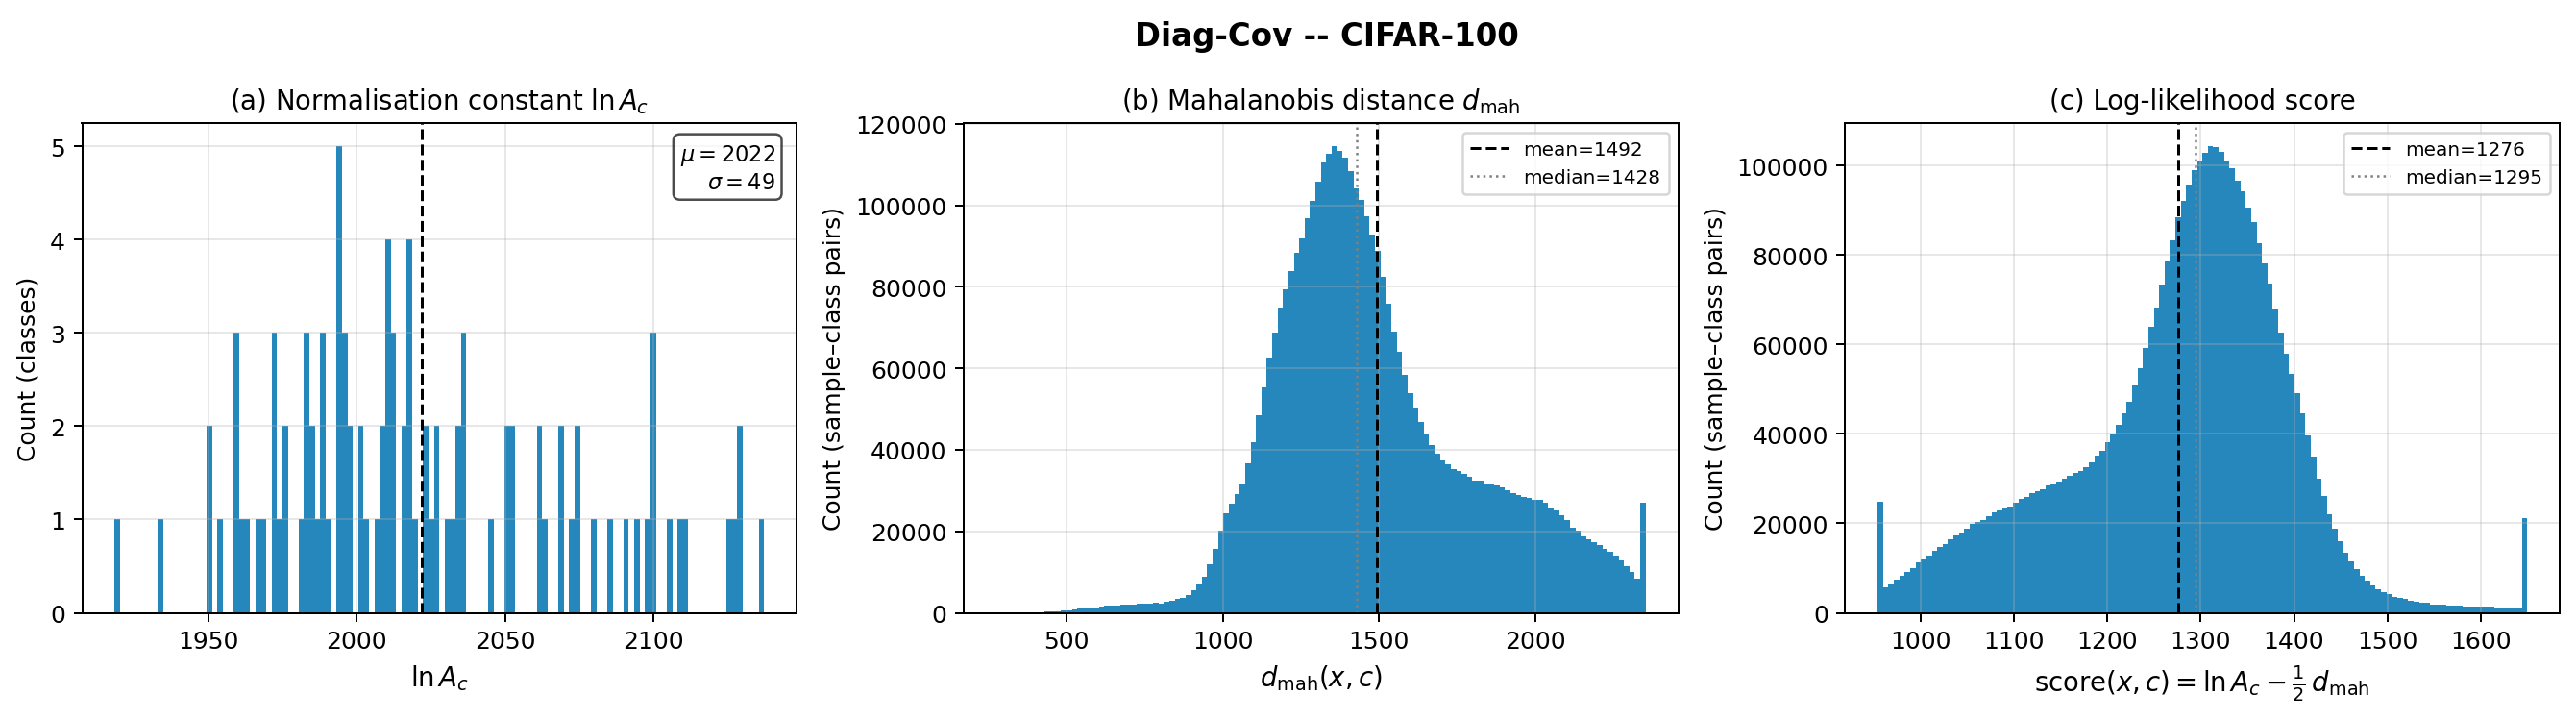
\includegraphics[width=0.99\linewidth]{imagenes/results/hist_scores_CIFAR100_train.png}
	\caption{\textbf{CIFAR-100 --- Training set} (Diag-Cov). Empirical distributions of the volume term $\ln A_c$, the shape term $d_{\mathrm{mah}}$, and the final log-likelihood score, computed on the data used to fit the Gaussian parameters.}
	\label{fig:hist_cifar_train}
\end{figure}

\begin{figure}[htbp]
	\centering
	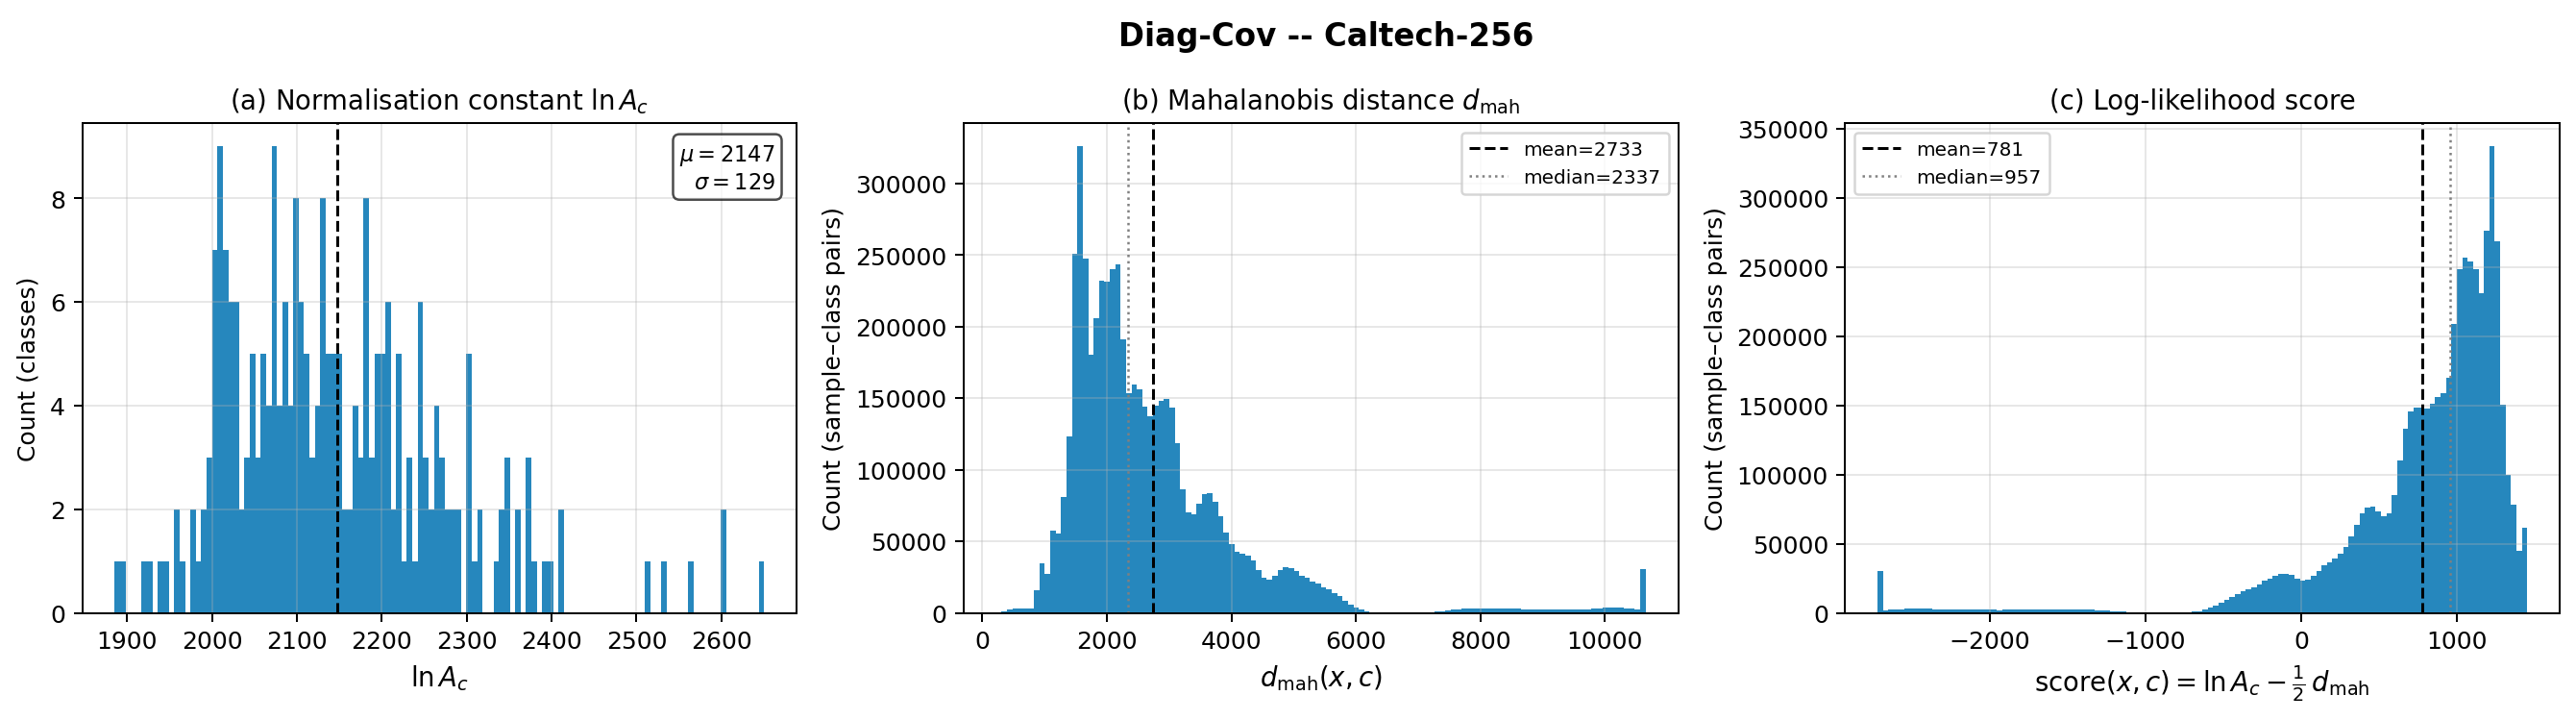
\includegraphics[width=0.99\linewidth]{imagenes/results/hist_scores_Caltech256_train.png}
	\caption{\textbf{Caltech-256 --- Training set} (Diag-Cov). Score component distributions on the training data.}
	\label{fig:hist_caltech_train}
\end{figure}

\begin{figure}[htbp]
	\centering
	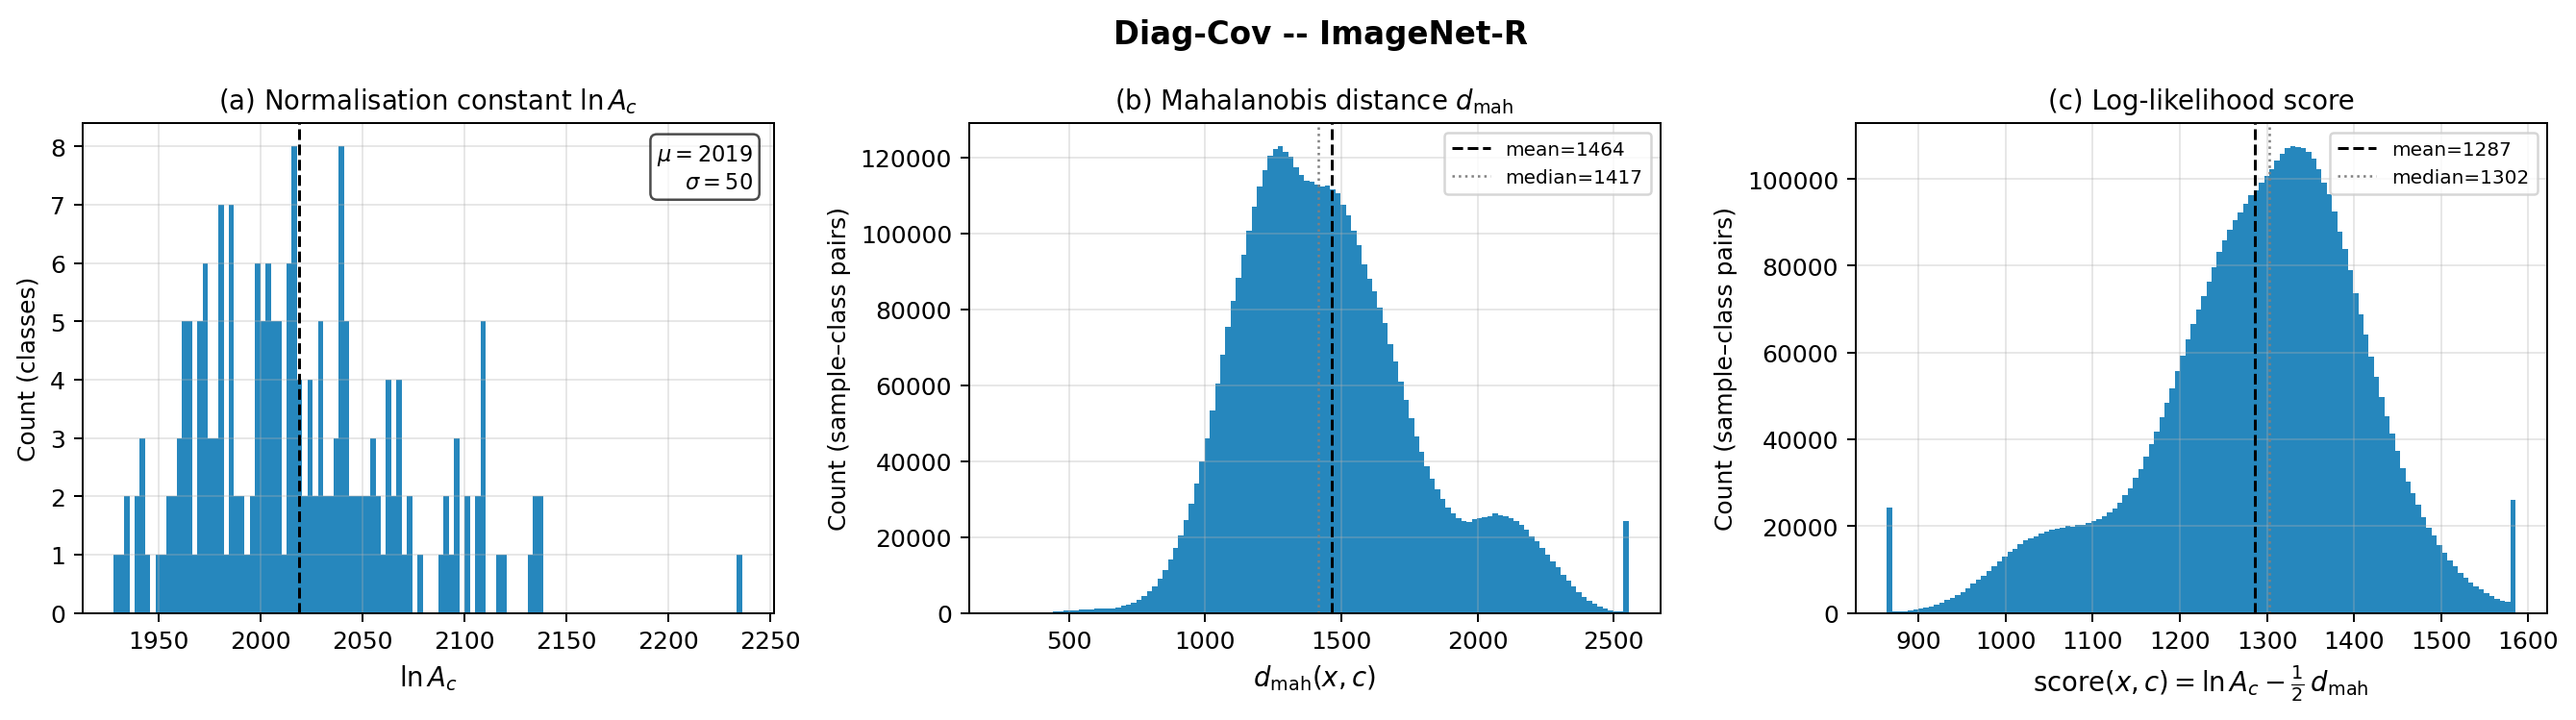
\includegraphics[width=0.99\linewidth]{imagenes/results/hist_scores_ImageNetR_train.png}
	\caption{\textbf{ImageNet-R --- Training set} (Diag-Cov). Score component distributions on the training data.}
	\label{fig:hist_imagenetr_train}
\end{figure}

% =============================================
% Diag-Cov: Validation splits (Caltech and ImageNet-R)
% =============================================

\section*{Diagonal Covariance --- Validation Splits (Caltech-256 and ImageNet-R)}

\begin{figure}[htbp]
	\centering
	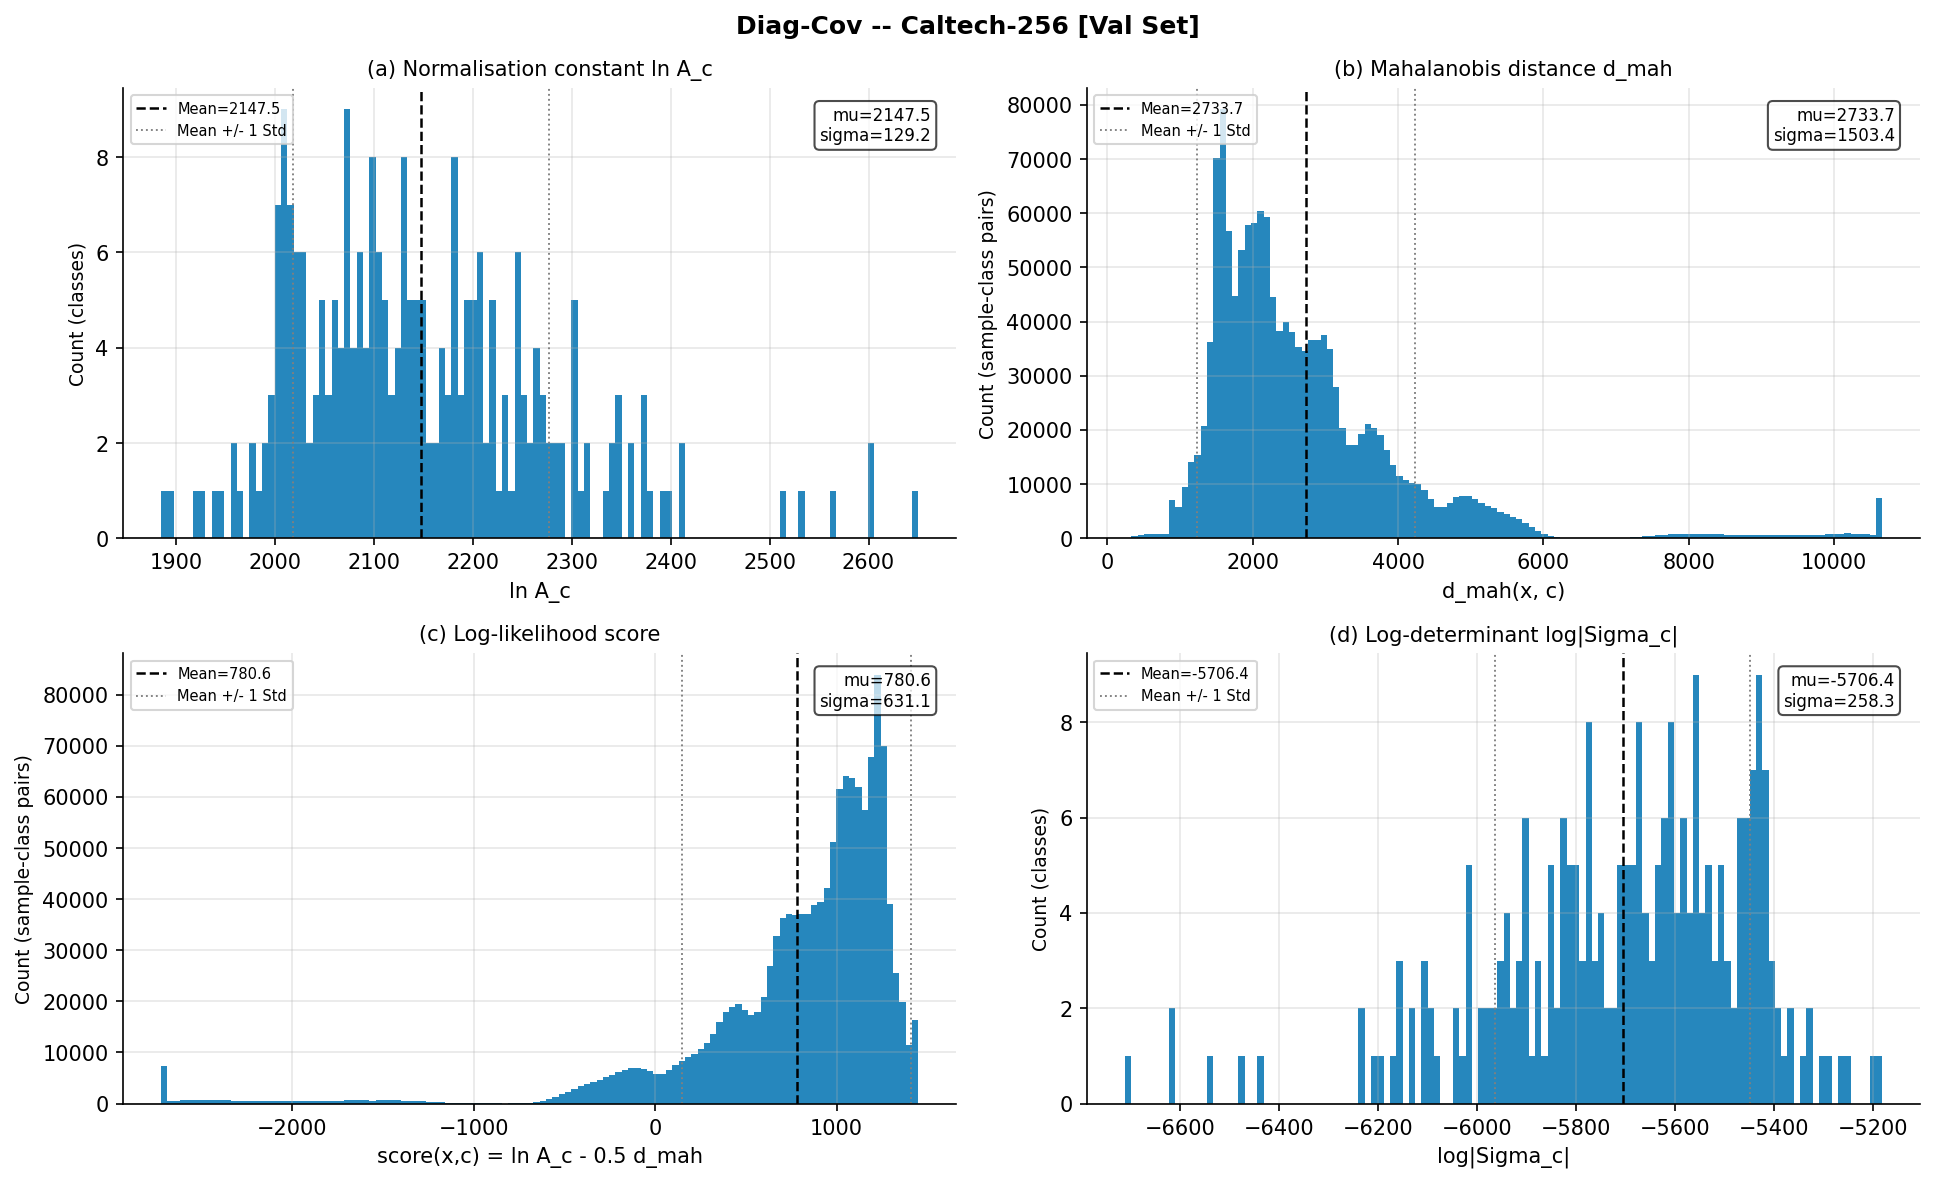
\includegraphics[width=0.99\linewidth]{imagenes/results/hist_scores_Caltech256_val.png}
	\caption{\textbf{Caltech-256 --- Validation set} (Diag-Cov). Score component distributions on held-out samples.}
	\label{fig:hist_caltech_val}
\end{figure}

\begin{figure}[htbp]
	\centering
	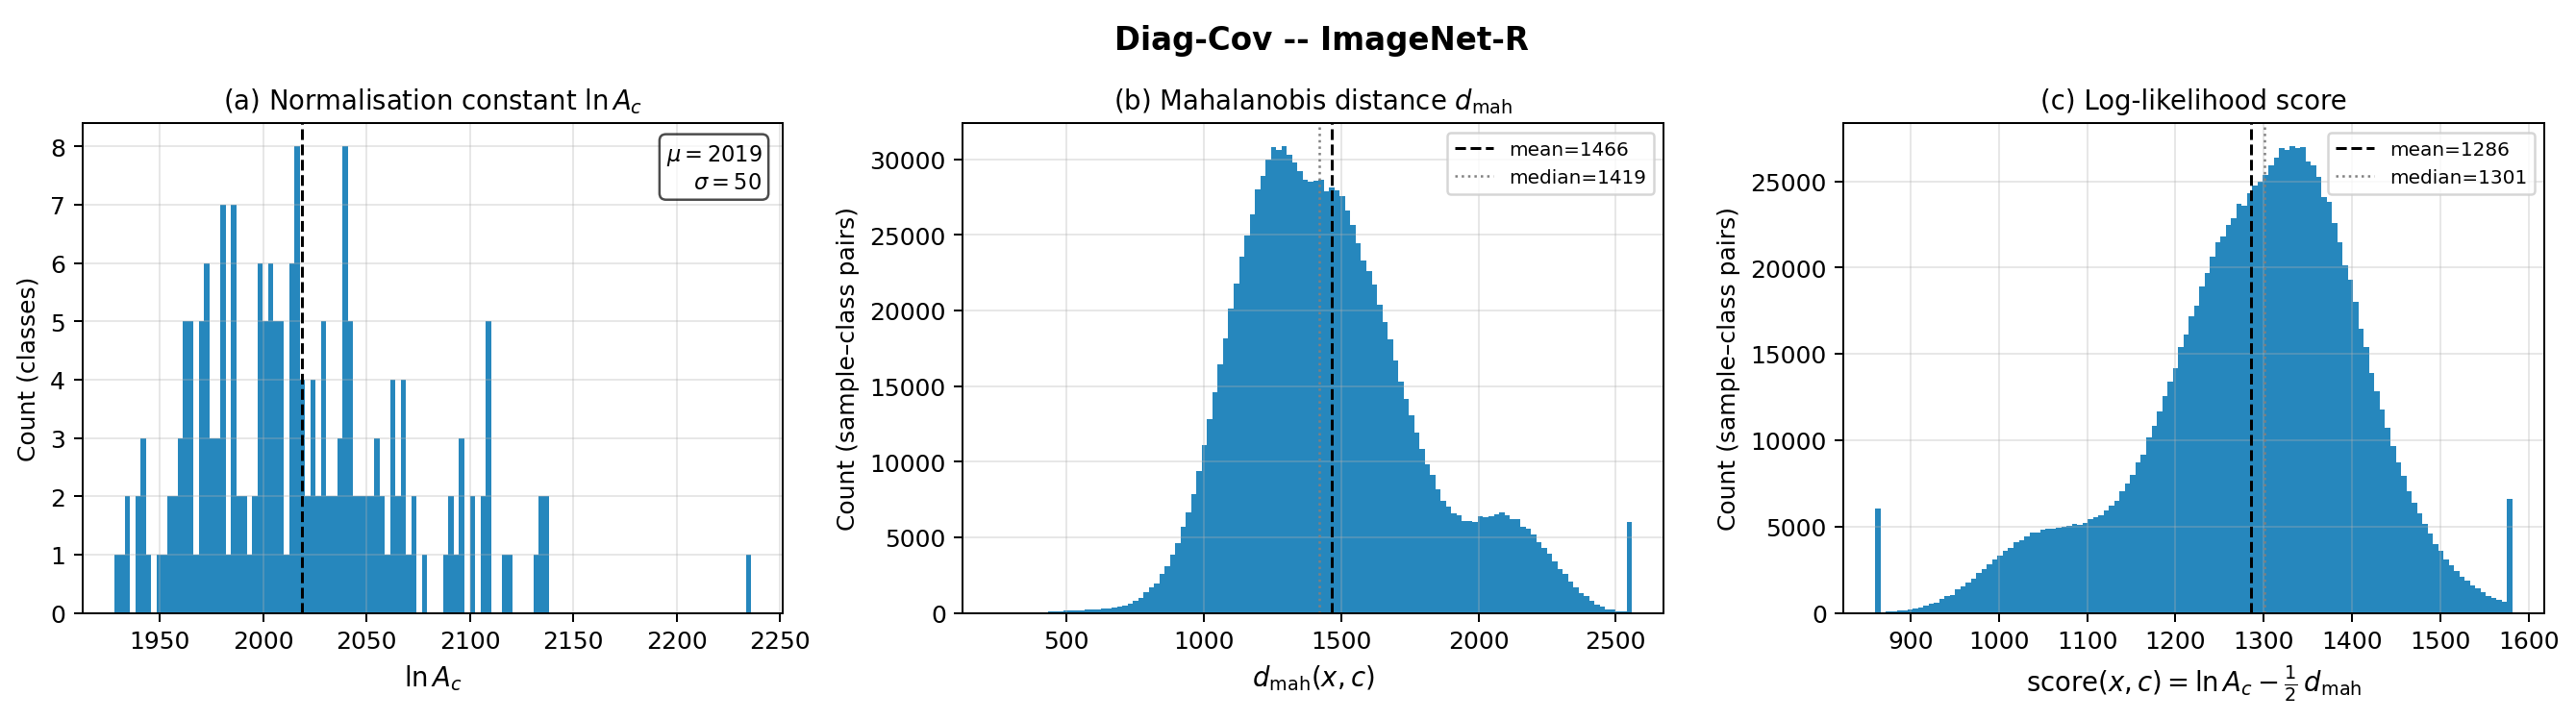
\includegraphics[width=0.99\linewidth]{imagenes/results/hist_scores_ImageNetR_val.png}
	\caption{\textbf{ImageNet-R --- Validation set} (Diag-Cov). Score component distributions on held-out samples.}
	\label{fig:hist_imagenetr_val}
\end{figure}

% =============================================
% Full-Cov: Training splits
% =============================================

\section*{Full Covariance --- Training Splits}

\begin{figure}[htbp]
	\centering
	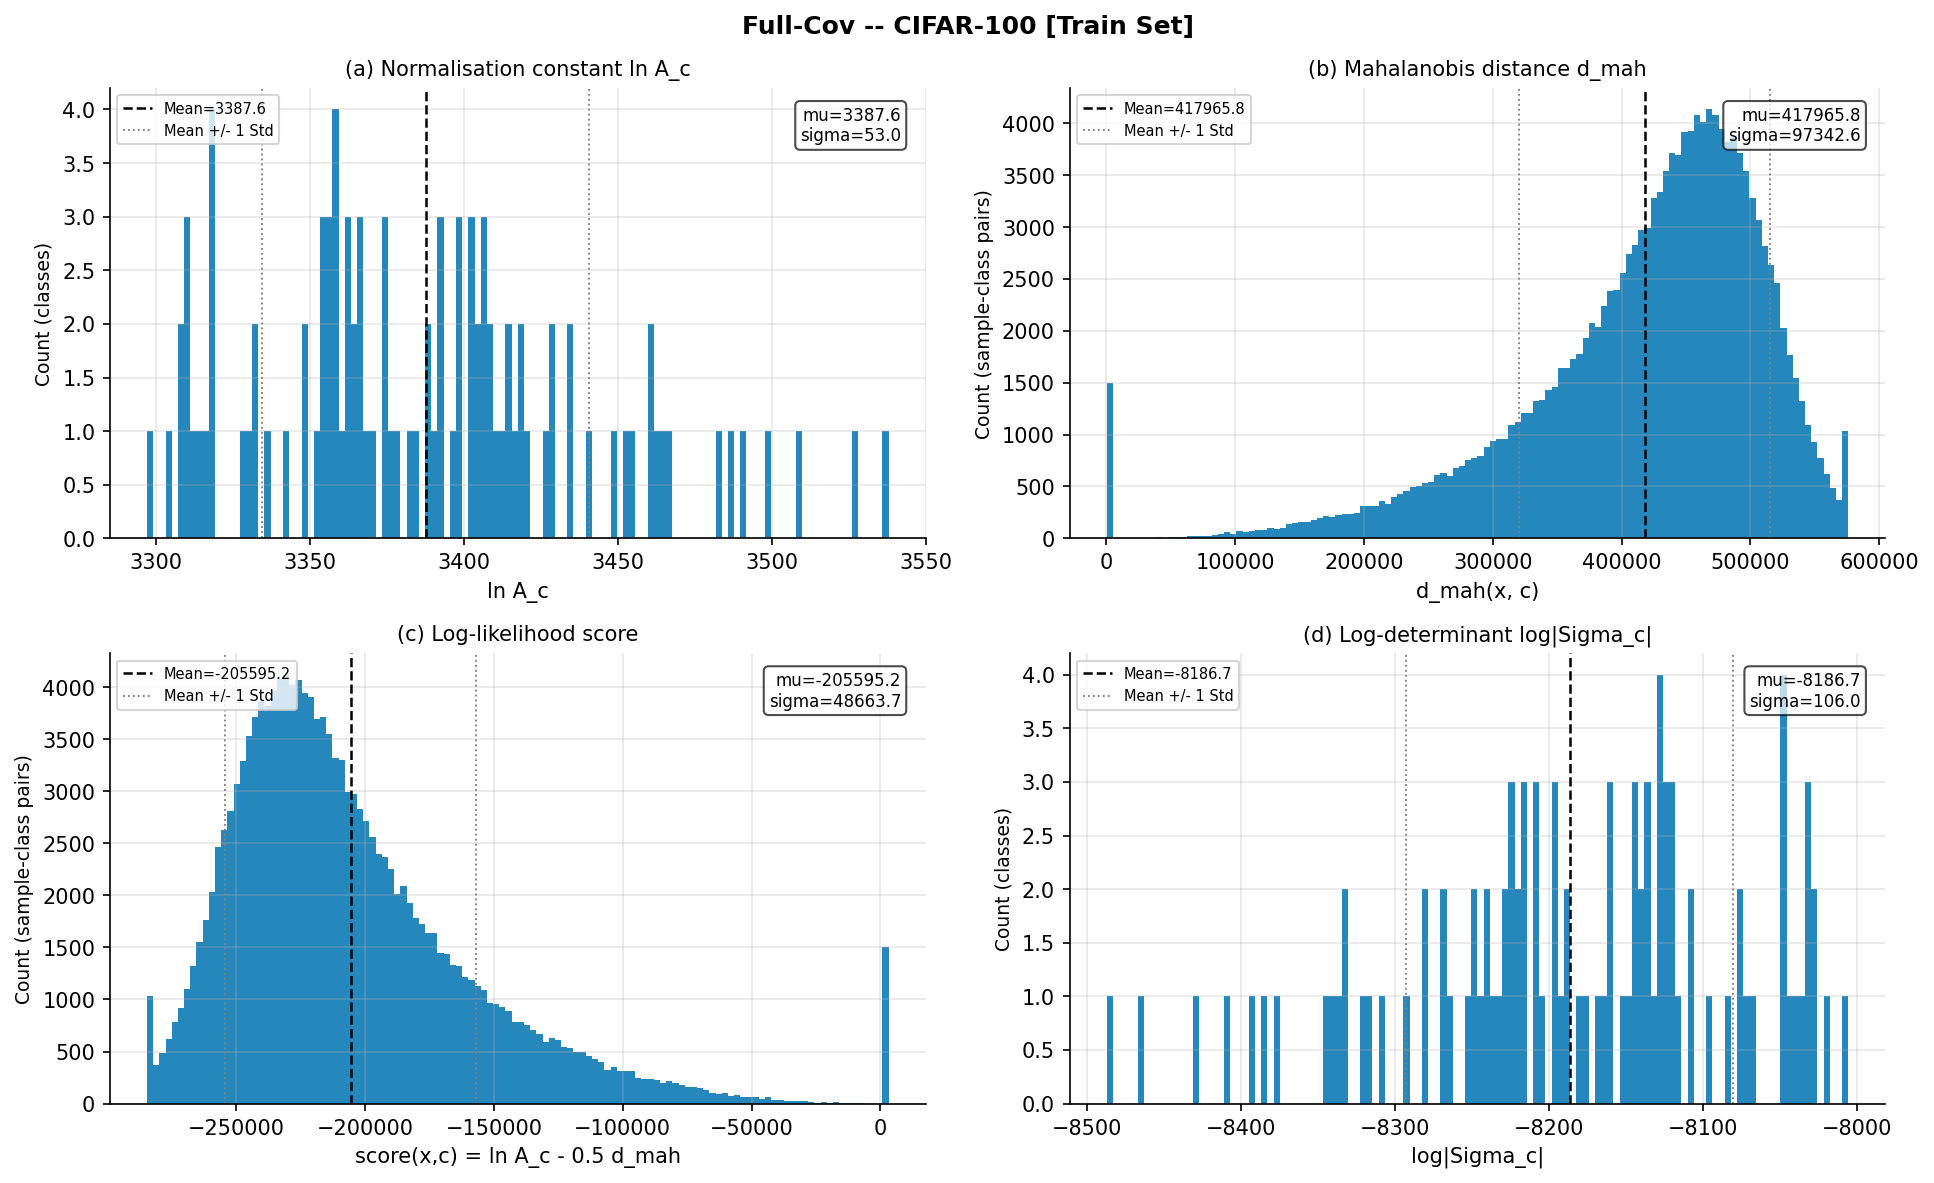
\includegraphics[width=0.99\linewidth]{imagenes/results/hist_scores_CIFAR100_train_full.png}
	\caption{\textbf{CIFAR-100 --- Training set} (Full-Cov). Score component distributions on the training data.}
	\label{fig:hist_cifar_train_full}
\end{figure}

\begin{figure}[htbp]
	\centering
	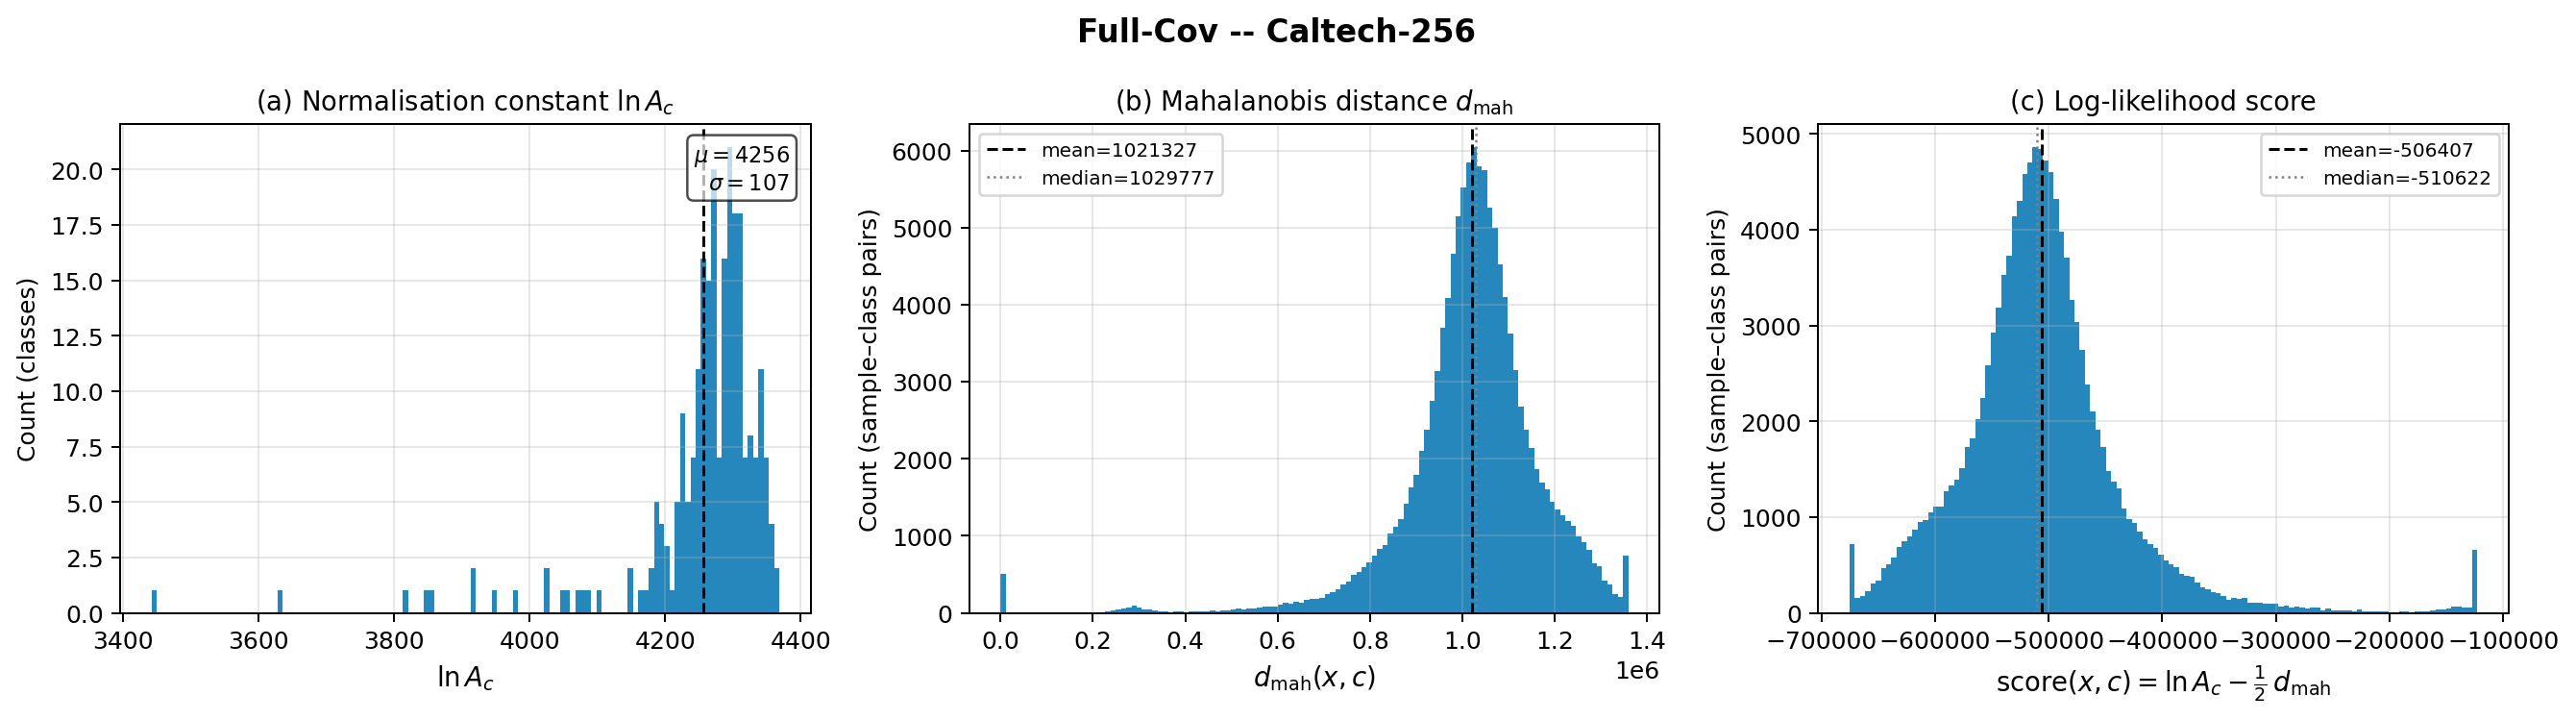
\includegraphics[width=0.99\linewidth]{imagenes/results/hist_scores_Caltech256_train_full.png}
	\caption{\textbf{Caltech-256 --- Training set} (Full-Cov). Score component distributions on the training data.}
	\label{fig:hist_caltech_train_full}
\end{figure}

\begin{figure}[htbp]
	\centering
	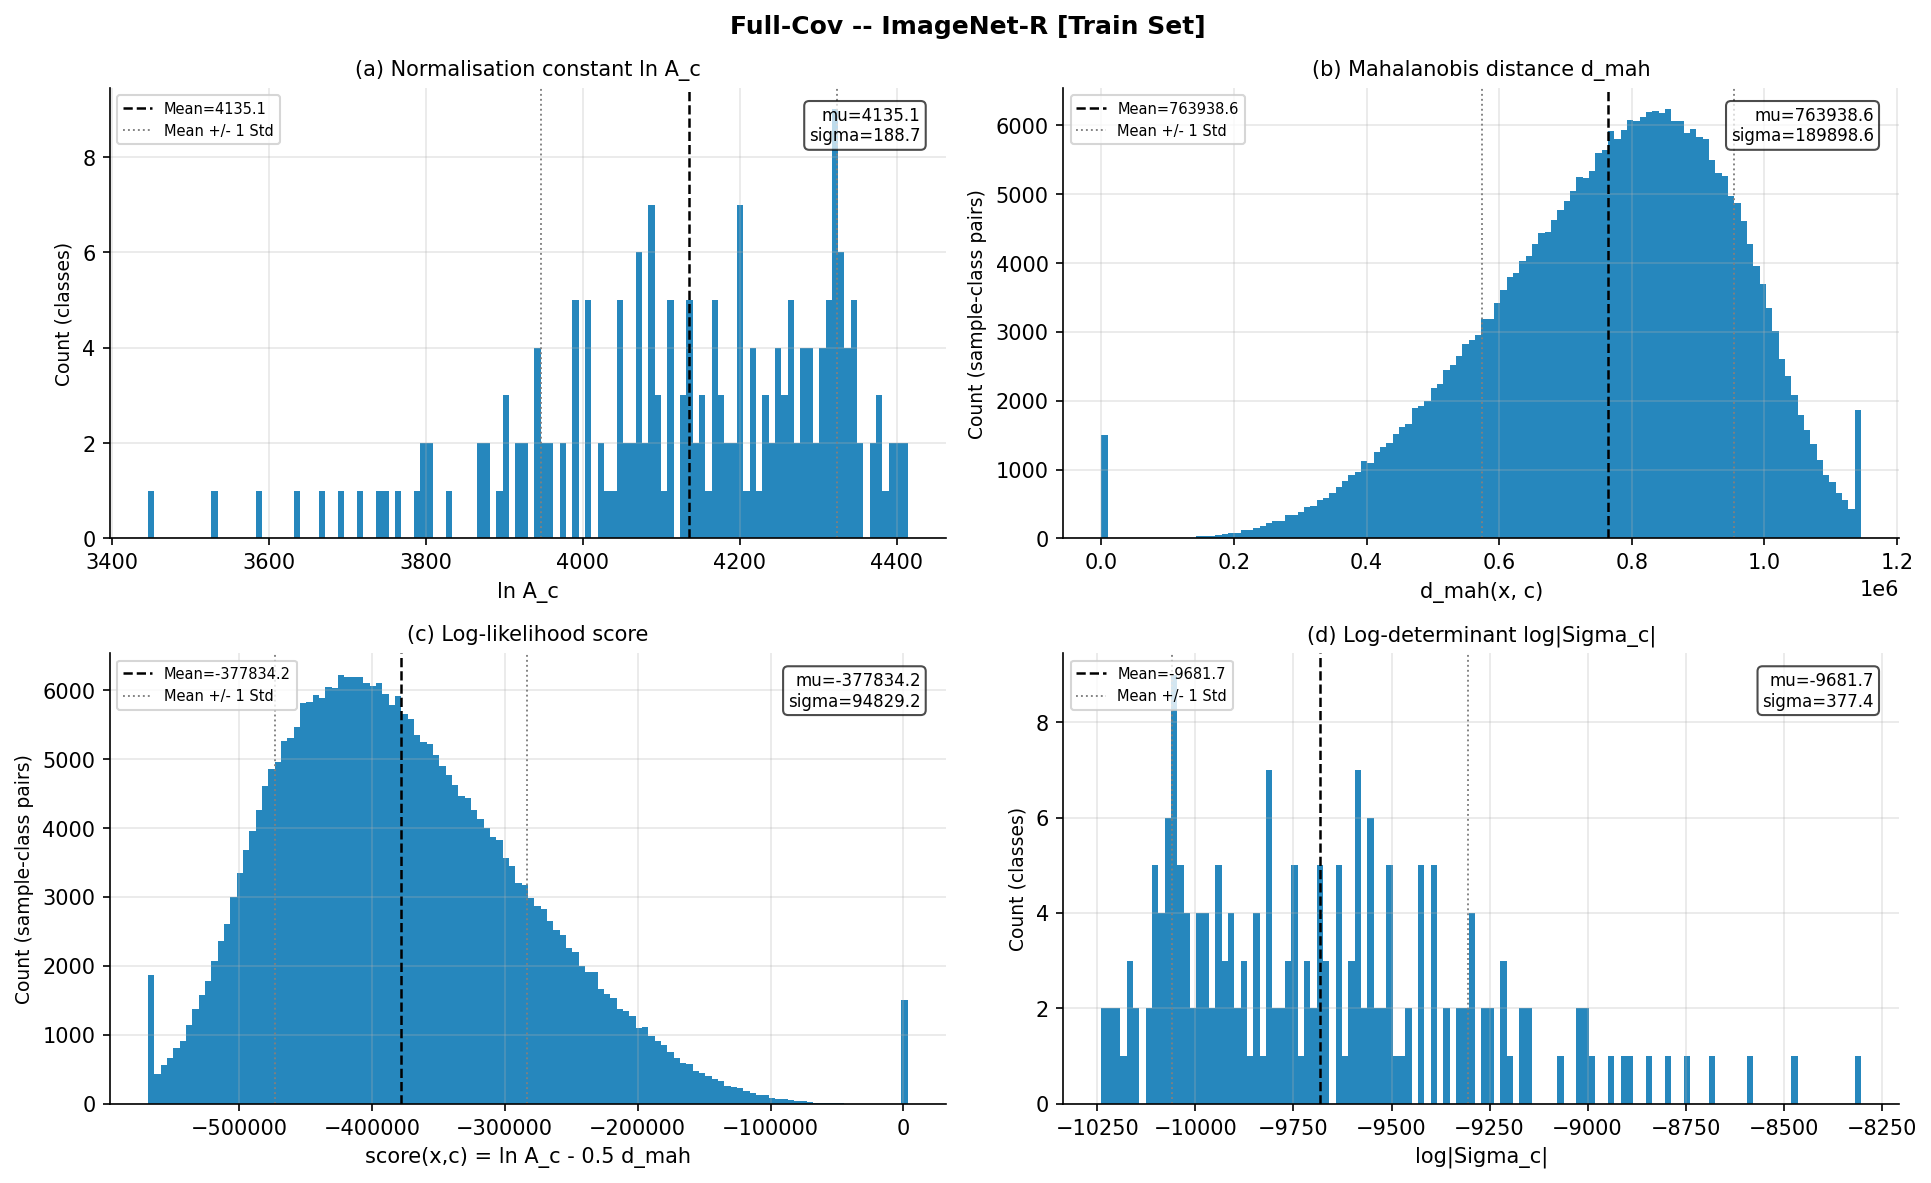
\includegraphics[width=0.99\linewidth]{imagenes/results/hist_scores_ImageNetR_train_full.png}
	\caption{\textbf{ImageNet-R --- Training set} (Full-Cov). Score component distributions on the training data.}
	\label{fig:hist_imagenetr_train_full}
\end{figure}

% =============================================
% Full-Cov: Validation splits (Caltech and ImageNet-R)
% =============================================

\section*{Full Covariance --- Validation Splits (Caltech-256 and ImageNet-R)}

\begin{figure}[htbp]
	\centering
	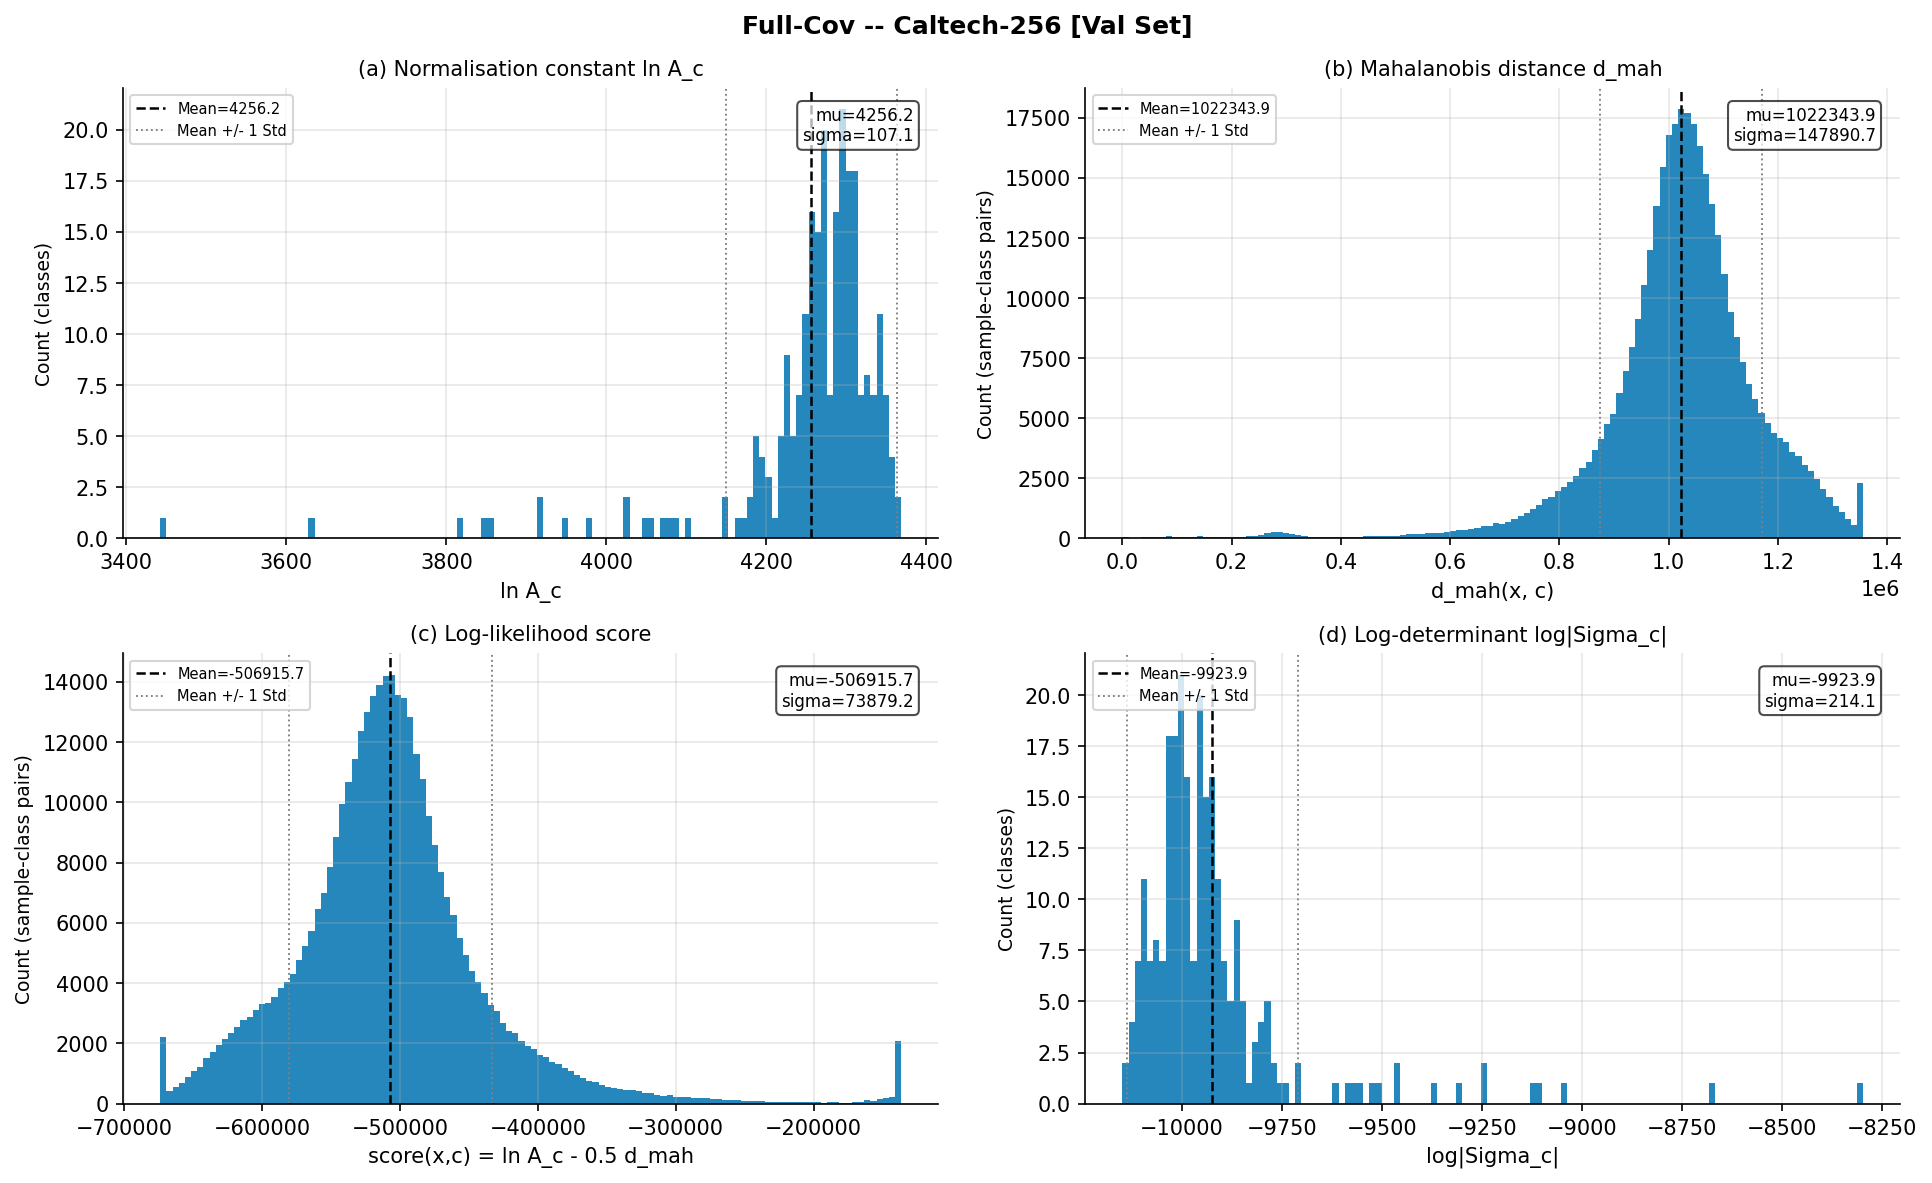
\includegraphics[width=0.99\linewidth]{imagenes/results/hist_scores_Caltech256_val_full.png}
	\caption{\textbf{Caltech-256 --- Validation set} (Full-Cov). Score component distributions on held-out samples.}
	\label{fig:hist_caltech_val_full}
\end{figure}

\begin{figure}[htbp]
	\centering
	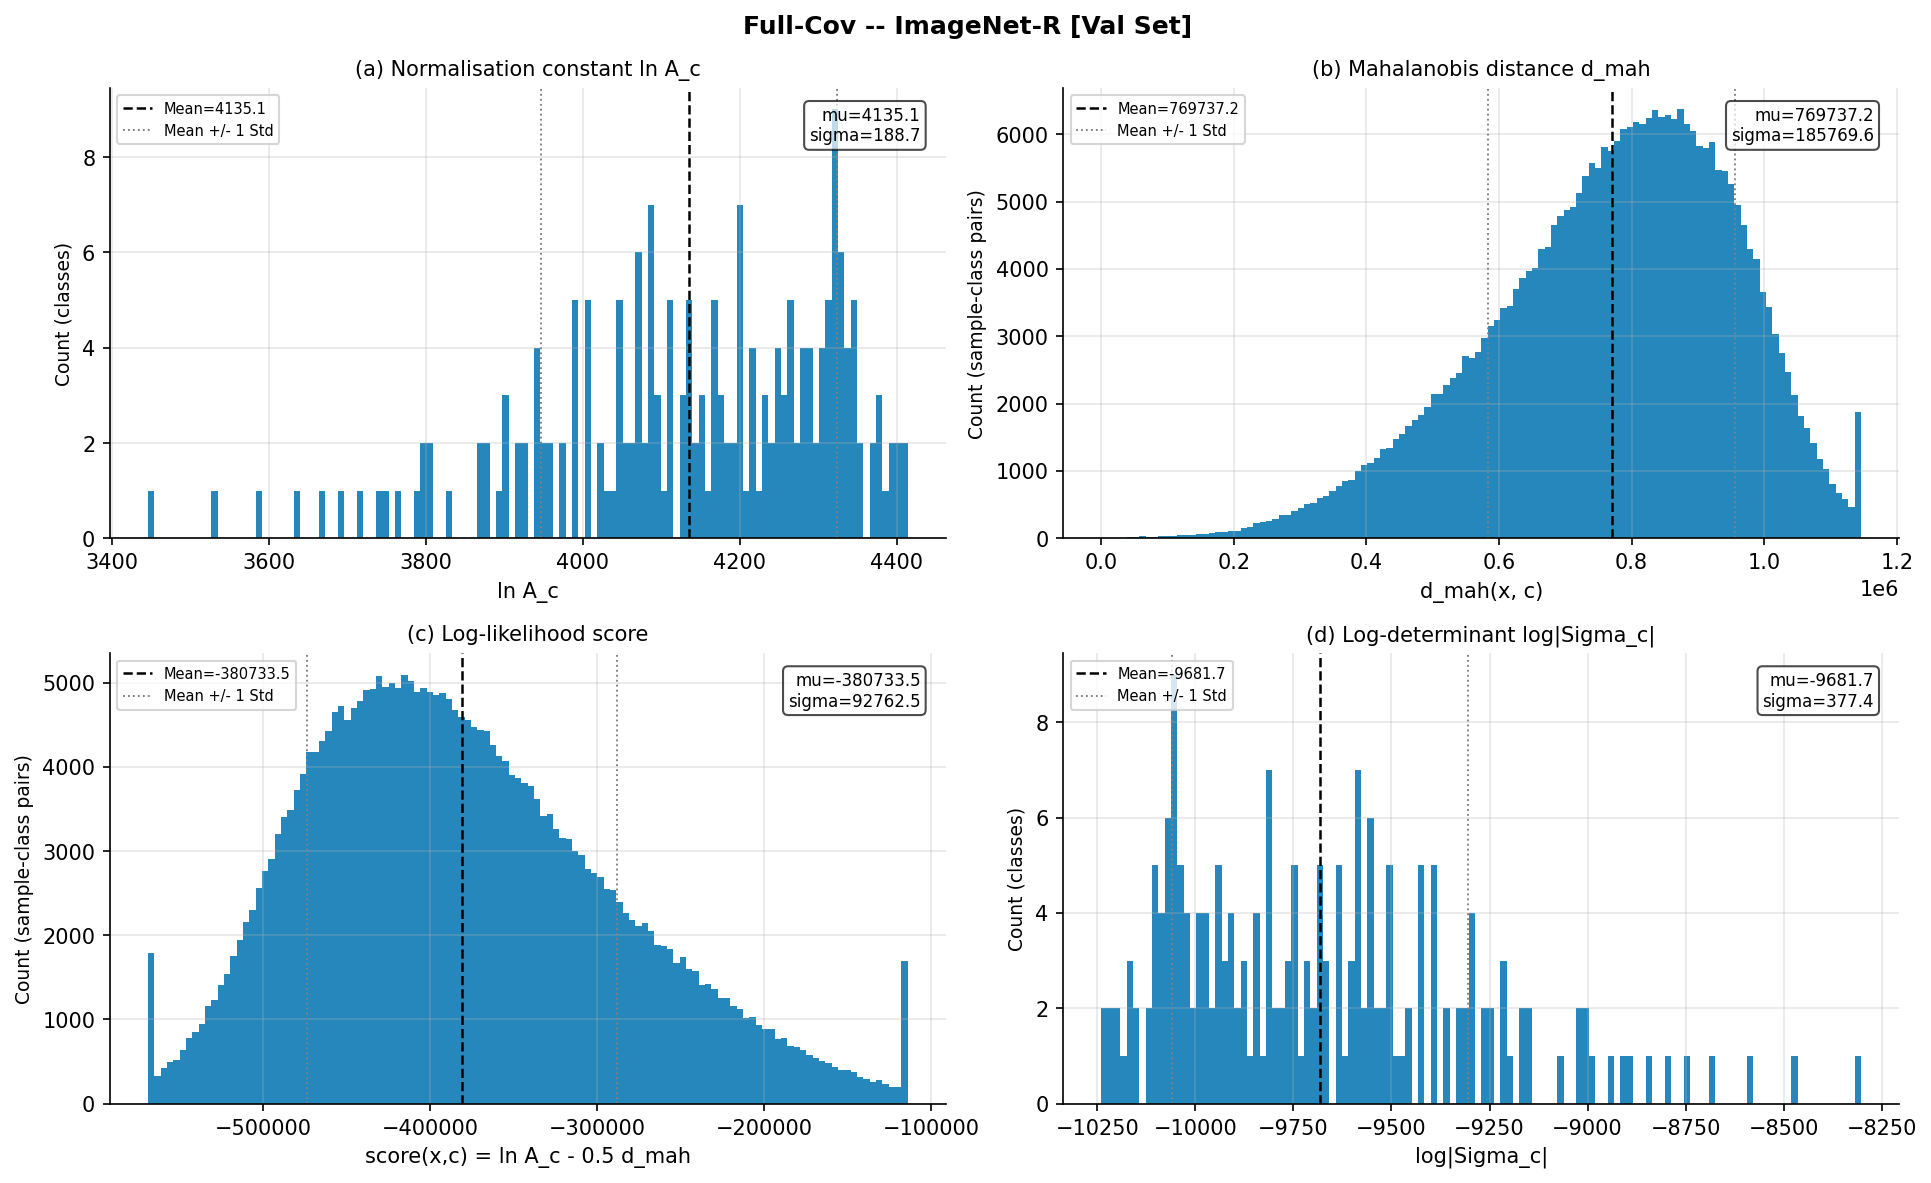
\includegraphics[width=0.99\linewidth]{imagenes/results/hist_scores_ImageNetR_val_full.png}
	\caption{\textbf{ImageNet-R --- Validation set} (Full-Cov). Score component distributions on held-out samples.}
	\label{fig:hist_imagenetr_val_full}
\end{figure}
